\chapter{Thiết kế hệ thống}

\section{Giới thiệu chương}

Sau khi hoàn thành quá trình phân tích yêu cầu hệ thống ở Chương 2, chương này trình bày thiết kế chi tiết của hệ thống AITasker. Nội dung bao gồm thiết kế kiến trúc tổng thể, thiết kế cơ sở dữ liệu, thiết kế API và thiết kế giao diện người dùng. Các nội dung được xây dựng nhằm đảm bảo hệ thống đáp ứng đầy đủ các yêu cầu chức năng và phi chức năng đã đề ra, đồng thời tạo nền tảng cho quá trình triển khai và kiểm thử ở các chương tiếp theo.

%====================================================

\section{Kiến trúc tổng thể hệ thống}

Hệ thống AITasker được xây dựng theo mô hình kiến trúc ba lớp (Three-Tier Architecture) bao gồm lớp giao diện, lớp xử lý nghiệp vụ và lớp dữ liệu.

Mô hình này giúp tách biệt các thành phần chức năng của hệ thống, tăng khả năng mở rộng, bảo trì và nâng cấp trong tương lai.

Các thành phần chính của hệ thống bao gồm:

\begin{itemize}
\item \textbf{Presentation Layer (Frontend):} Được xây dựng bằng ReactJS, cung cấp giao diện tương tác cho người dùng bao gồm doanh nghiệp, chuyên gia và quản trị viên.
\item \textbf{Business Layer (Backend):} Được phát triển bằng FastAPI, cung cấp các RESTful API xử lý nghiệp vụ của hệ thống.
\item \textbf{Data Layer (Database):} Sử dụng PostgreSQL để lưu trữ dữ liệu của hệ thống.
\item \textbf{Cloud Infrastructure:} Hệ thống được triển khai trên nền tảng Azure Cloud nhằm đảm bảo khả năng mở rộng và tính sẵn sàng cao.
\item \textbf{Storage Service:} Azure Blob Storage được sử dụng để lưu trữ hình ảnh hồ sơ, tệp đính kèm và tài liệu dự án.
\end{itemize}

\begin{figure}[H]
\centering
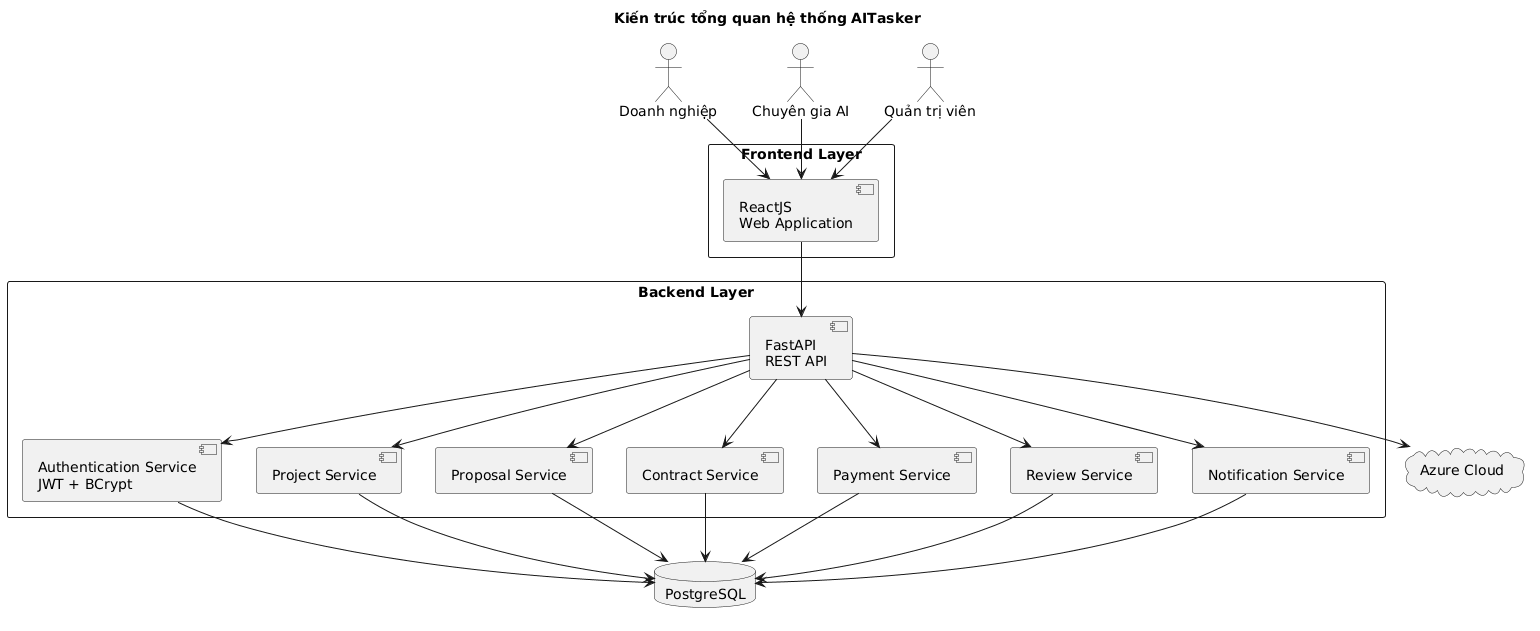
\includegraphics[width=\textwidth]{figures/architecture.png}
\caption{Kiến trúc tổng thể hệ thống AITasker}
\label{fig:architecture}
\end{figure}

%====================================================

\section{Thiết kế cơ sở dữ liệu}

\subsection{Tổng quan cơ sở dữ liệu}

Hệ thống sử dụng PostgreSQL làm hệ quản trị cơ sở dữ liệu quan hệ. Cơ sở dữ liệu được thiết kế dựa trên mô hình Entity Relationship Diagram (ERD) nhằm đảm bảo tính toàn vẹn dữ liệu và khả năng mở rộng.

Các bảng dữ liệu được chuẩn hóa nhằm giảm thiểu sự dư thừa và đảm bảo tính nhất quán của dữ liệu.

\subsection{Các thực thể chính}

\begin{table}[H]
\centering
\caption{Danh sách các thực thể chính}
\begin{tabular}{|p{4cm}|p{9cm}|}
\hline
\textbf{Thực thể} & \textbf{Mô tả} \\
\hline
Users & Quản lý thông tin tài khoản người dùng. \\
\hline
Enterprises & Quản lý thông tin doanh nghiệp. \\
\hline
Experts & Quản lý hồ sơ chuyên gia. \\
\hline
Skills & Danh sách kỹ năng chuyên môn. \\
\hline
Expert\_Skills & Liên kết kỹ năng với chuyên gia. \\
\hline
Categories & Danh mục dự án. \\
\hline
Projects & Thông tin dự án được đăng tải. \\
\hline
Project\_Files & Tệp đính kèm của dự án. \\
\hline
Proposals & Đề xuất của chuyên gia gửi cho dự án. \\
\hline
Contracts & Hợp đồng giữa doanh nghiệp và chuyên gia. \\
\hline
Milestones & Các giai đoạn thực hiện hợp đồng. \\
\hline
Payments & Thông tin thanh toán. \\
\hline
Conversations & Cuộc trò chuyện giữa các bên. \\
\hline
Messages & Tin nhắn trong cuộc trò chuyện. \\
\hline
Reviews & Đánh giá sau khi hoàn thành dự án. \\
\hline
Notifications & Thông báo hệ thống. \\
\hline
\end{tabular}
\end{table}

\subsection{Biểu đồ ERD}

\begin{figure}[H]
\centering

\includegraphics[width=\textwidth]{figures/ERD.png}
\caption{Biểu đồ thực thể liên kết (ERD)}
\label{fig:erd}
\end{figure}

%====================================================

\section{Thiết kế API}

Hệ thống sử dụng kiến trúc RESTful API để trao đổi dữ liệu giữa Frontend và Backend.

Các API được phân chia theo từng nhóm chức năng nhằm thuận tiện cho việc phát triển và bảo trì hệ thống.

\subsection{API xác thực}

\begin{table}[H]
\centering
\caption{Nhóm API xác thực}
\begin{tabular}{|c|p{6cm}|p{5cm}|}
\hline
Method & Endpoint & Chức năng \\
\hline
POST & /auth/register & Đăng ký tài khoản \\
\hline
POST & /auth/login & Đăng nhập hệ thống \\
\hline
GET & /auth/profile & Lấy thông tin người dùng \\
\hline
PUT & /auth/profile & Cập nhật hồ sơ cá nhân \\
\hline
\end{tabular}
\end{table}

\subsection{API dự án}

\begin{table}[H]
\centering
\caption{Nhóm API quản lý dự án}
\begin{tabular}{|c|p{6cm}|p{5cm}|}
\hline
Method & Endpoint & Chức năng \\
\hline
GET & /projects & Danh sách dự án \\
\hline
POST & /projects & Tạo dự án mới \\
\hline
GET & /projects/\{id\} & Chi tiết dự án \\
\hline
PUT & /projects/\{id\} & Cập nhật dự án \\
\hline
DELETE & /projects/\{id\} & Xóa dự án \\
\hline
\end{tabular}
\end{table}

\subsection{API đề xuất}

\begin{table}[H]
\centering
\caption{Nhóm API quản lý đề xuất}
\begin{tabular}{|c|p{6cm}|p{5cm}|}
\hline
Method & Endpoint & Chức năng \\
\hline
POST & /proposals & Gửi đề xuất \\
\hline
GET & /proposals & Danh sách đề xuất \\
\hline
PUT & /proposals/\{id\} & Cập nhật trạng thái đề xuất \\
\hline
\end{tabular}
\end{table}

\subsection{API hợp đồng và thanh toán}

\begin{table}[H]
\centering
\caption{Nhóm API hợp đồng và thanh toán}
\begin{tabular}{|c|p{6cm}|p{5cm}|}
\hline
Method & Endpoint & Chức năng \\
\hline
POST & /contracts & Tạo hợp đồng \\
\hline
GET & /contracts & Danh sách hợp đồng \\
\hline
POST & /payments & Thanh toán hợp đồng \\
\hline
GET & /payments & Danh sách giao dịch \\
\hline
\end{tabular}
\end{table}

%====================================================

\section{Thiết kế giao diện người dùng}

Giao diện người dùng được xây dựng theo mô hình Single Page Application (SPA) sử dụng ReactJS nhằm nâng cao trải nghiệm người dùng và giảm thời gian tải trang.

Các màn hình chính của hệ thống bao gồm:

\begin{itemize}
\item Trang chủ.
\item Trang đăng ký tài khoản.
\item Trang đăng nhập.
\item Trang hồ sơ doanh nghiệp.
\item Trang hồ sơ chuyên gia.
\item Trang danh sách dự án.
\item Trang chi tiết dự án.
\item Trang gửi đề xuất.
\item Trang quản lý hợp đồng.
\item Trang thanh toán.
\item Trang đánh giá.
\item Trang thông báo.
\item Trang quản trị hệ thống.
\end{itemize}

%====================================================

\section{Thiết kế bảo mật hệ thống}

Để đảm bảo an toàn dữ liệu và bảo mật thông tin người dùng, hệ thống áp dụng các cơ chế bảo mật sau:

\begin{itemize}
\item Xác thực người dùng bằng JWT (JSON Web Token).
\item Mã hóa mật khẩu bằng BCrypt.
\item Phân quyền theo vai trò (Role-Based Access Control).
\item Sử dụng giao thức HTTPS khi truyền dữ liệu.
\item Kiểm tra dữ liệu đầu vào nhằm ngăn chặn SQL Injection và XSS.
\item Giới hạn quyền truy cập đối với các API quan trọng.
\end{itemize}

%====================================================

\section{Kết luận chương}

Chương này đã trình bày thiết kế tổng thể của hệ thống AITasker bao gồm kiến trúc hệ thống, thiết kế cơ sở dữ liệu, thiết kế API, giao diện người dùng và các cơ chế bảo mật. Những nội dung này là cơ sở để triển khai hệ thống thực tế và thực hiện kiểm thử trong các chương tiếp theo.